\documentclass{ctexart}
\usepackage[left=1.5cm,right=1.5cm,top=1.5cm,bottom=1.5cm]{geometry}
\usepackage{listings}
\usepackage[dvipsnames]{xcolor}
\usepackage{cite}
\usepackage{diagbox}
\usepackage{fancyhdr} % 加载fancyhdr宏包,用于设置页眉和页脚
\pagestyle{fancy} % 设置页面样式
\fancyhf{} % 清除默认的页眉和页脚的内容
\fancyfoot[C]{\thepage} 
\renewcommand{\headrulewidth}{0pt} % 将页眉的横线宽度设置为0pt

\usepackage{graphicx}
\usepackage{longtable}
\usepackage{tabularx}
\usepackage{float}
\usepackage{amsmath}%引用宏包要放在documentclass后面,否则报错
\usepackage{hyperref}
\usepackage{bm}
\usepackage{amssymb}
\usepackage{esint}
\usepackage{booktabs}
%\usepackage{subfiles}%用于分章节管理引用,使各章节引用来源于各自的文件,编号相互独立
\usepackage{amsthm}
\title{数字电路实验\quad 实验报告9}
\author{Leo}
\date{\today}
\begin{document}
\maketitle
\section{实验内容}
设计四路抢答器:\\
1.熟悉触发器,时序计数器,组合逻辑,译码显示等单元\\
2.列出状态转移真值表和转换图 \\
3.给出电路实现方案\\
4.调试电路,实现抢答用消抖动开关实现,能判断出抢答的同时,排斥其他组输入的干扰,封闭其他各路输入、使其他组再按开关时无效,对抢中者用声、光显示,主持人设有开始、清除按键复位系统。\\
5.扩展:加设回答计时功能,显示精确到秒,最长限时为30秒\\
\section{实验器材}
Pocketlab、电脑、导线若干、镊子、限流电阻8个、绿色LED灯4个、7400*1、7404*1、7420*1、74191*1、7448*1、7474*2、7段数码管*1。芯片的引脚图如下所示
\begin{figure}[H]
    \centering
    \begin{minipage}{0.45\textwidth}
    \centering
           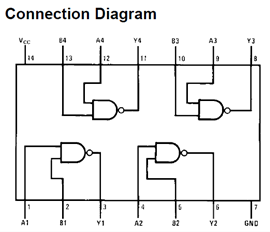
\includegraphics[width=0.6\textwidth]{7400.png}
           \caption{7400}
    \label{}
    \end{minipage}
    \hspace{0.05\textwidth}
    \begin{minipage}{0.45\textwidth}
    \centering
           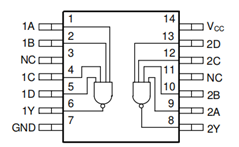
\includegraphics[width=0.6\textwidth]{7420.png}
           \caption{7420}
    \label{7474}
    \end{minipage}
\end{figure}
\begin{figure}[H]
    \centering
    \begin{minipage}{0.5\textwidth}
    \centering
           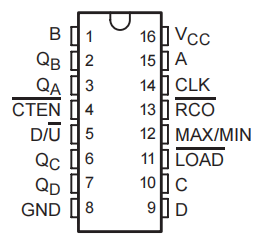
\includegraphics[width=0.5\textwidth]{74191.png}
           \caption{74191}
    \label{}
    \end{minipage}
    \hspace{0.05\textwidth}
    \begin{minipage}{0.4\textwidth}
    \centering
           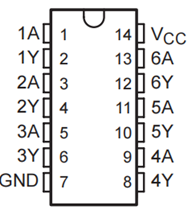
\includegraphics[width=0.5\textwidth]{7404.png}
           \caption{7404}
    \label{7474}
    \end{minipage}
\end{figure}
\begin{figure}[H]
    \centering
    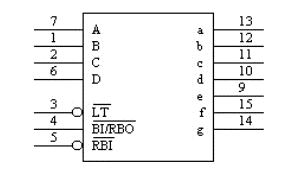
\includegraphics[width=0.25\textwidth]{7448.png}
    \caption{7448}
\end{figure}
\section{实验原理}
\subsection{消抖电路的设计}
根据教材第181页的阐述,可以用RS锁存器来实现机械开关的消抖电路。对于4路输入而言每个消抖电路都一样,所以这里只需要分析一次。仿照用与非门组成的基本RS锁存器,加上一个单刀双掷开关可以构成如图所示的消抖电路
\begin{figure}[H]
    \centering
    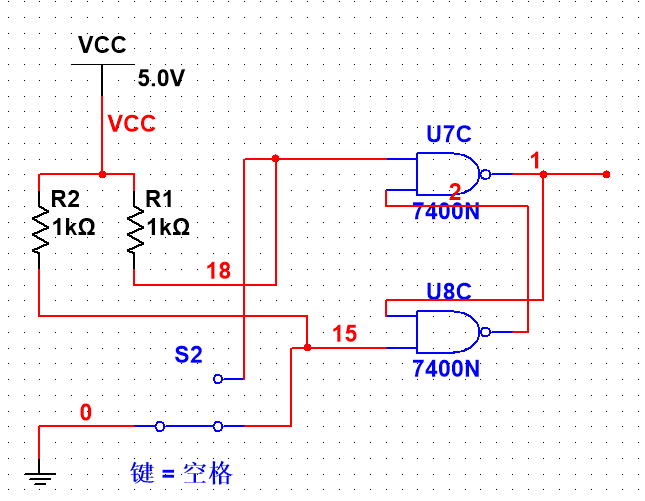
\includegraphics[width=0.5\textwidth]{消抖电路.png}
    \caption{消抖电路}
\end{figure}
当开关与上面的与非门相连的时候,上与非门有一个输入为0,导致输出结果为1;当开关与下面的与非门相连的时候,下与非门有一个输入为0,使得上与非门的两个输入均为1,结果输出为0.注意:这里的电阻是不可省去的,否则不管开关在什么位置,高电平始终直接接到地,造成短路。下面给出该锁存器的功能表
\begin{table}[H]
    \centering
    \caption{RS锁存器功能表}
    \begin{tabular}{cc|c}
    \hline 
        $S' $& $R'$ & $Q^{n+1}$ \\ \hline
        1 & 1 & $Q^{n}$ \\ \hline
        0 & 1 & 1 \\ \hline
        1 & 0 & 0 \\ \hline
        0 & 0 & 1(同态) \\ \hline
    \end{tabular}
    \label{RS锁存器功能表}
\end{table}
\subsection{屏蔽除第一位外其他各路输入的设计}
为了实现模块化的电路设计,不选择在锁存器部分加入屏蔽功能,使而是用D触发器,将D触发器的输出给到灯的输入端。同时,利用D触发器仅在时钟上升沿时刻更新数据的特点,通过控制时钟端输入来实现屏蔽除第一位外其他各路输入。只要我们用第一路到来的高电平将时钟信号屏蔽,就能屏蔽其他各路输入。对四路触发器的输出$Q_AQ_BQ_CQ_D$,考虑构造函数
\begin{align}
    F_1&=Q_A+Q_B+Q_C+Q_D\\
    CLK_1&=(CLK\cdot F_1')'
\end{align}
将$CLK_1$送到四个触发器的时钟端。这样,当有一个触发器的输出变为1(对应的指示灯亮)时,$F_1=CLK_1=1$,所有D触发器都得不到上升沿,保持在原状态。这样就能实现第一个输入屏蔽其他各路输入了。
\subsection{开始与清除按钮的设计}
为了实现模块化的电路设计,我们同样不选择在锁存器部分加入清零控制端,而是在触发器部分施加清零控制。将每个触发器的清零端与清零开关相连,实现当清零开关断开时清零端接到地,而当清零开关闭合时,清零端接到高电平。倒计时模块的清零在下一节另作说明。
\subsection{回答倒计时的设计}
假设回答不能超过9秒,采用倒计时的形式,很自然地想到利用同步二进制计数器向下计数的功能。为了从9开始计时,需要预先置数,这里采用同步置数的方法,将置数端设为常量1001,并将控制置数端LOAD'与主持人的清零按钮相连,使得当主持人按下按钮时,可以在把D触发器清零的同时,将计数器的初值设置为9。另外,按照常理,回答倒计时应该在选手抢答成功的同时开始计时。根据上一节的分析,当有指示灯亮起时,$F_1=1$,而在其他时候,$F_1=0$。利用这一特性,构造函数$CLK_2=(F_1\cdot CLK)'$给到计数器的时钟端。

设计好计数器后将计数器的输出与显示译码器7448连接,将动态灭零信号与试灯信号置为无效,再将7448输出端与7段数码管连接即可。
\section{电路实现与调试}
在Multisim中搭建电路。电路图如图所示,从左到右依次是:消抖电路、D触发器层、抢答成功提示灯和倒计时显示电路
\begin{figure}[H]
    \centering
    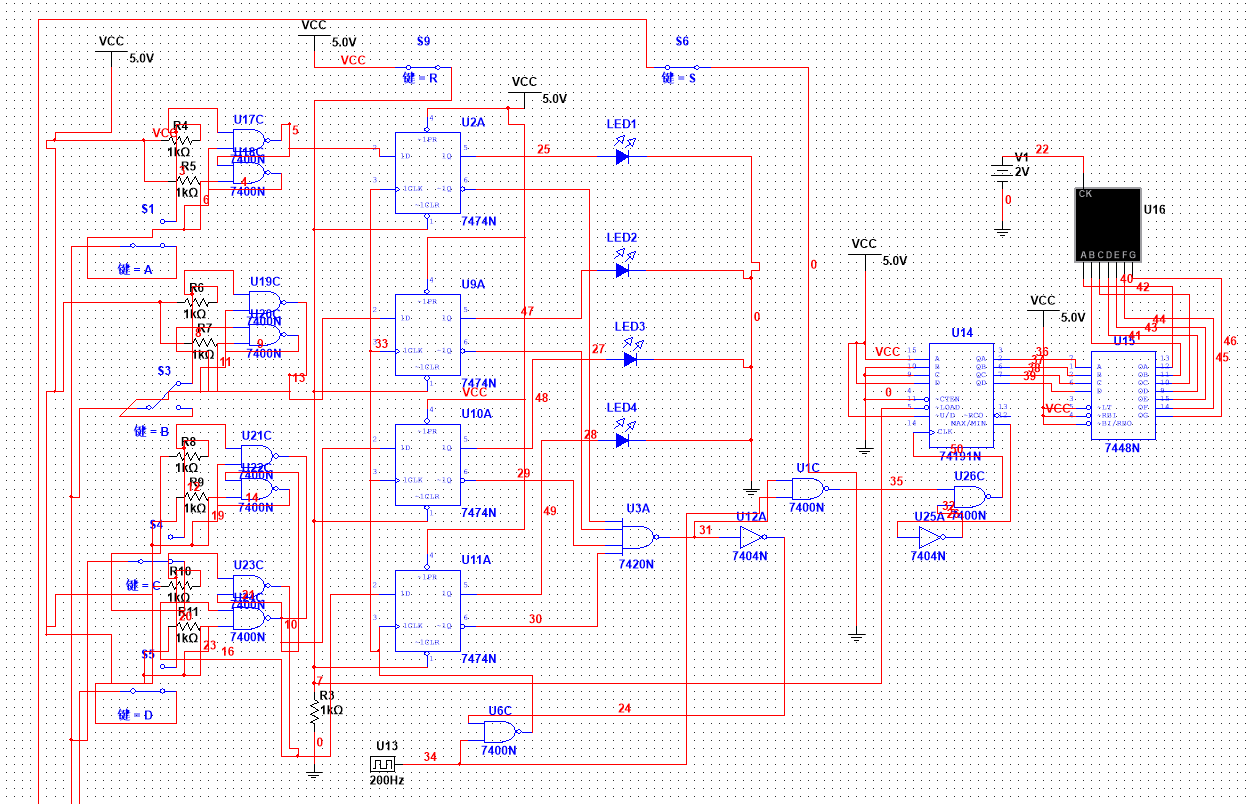
\includegraphics[width=0.8\textwidth]{multisim.png}
    \caption{multisim电路仿真图}
\end{figure}
下面搭建实物电路,如图所示
\begin{figure}[H]
    \centering
    \includegraphics[width=0.8\textwidth]{实物电路图.jpg}
    \caption{实物电路图}
\end{figure}
最左上角为主持人开始按钮,最右边是清零按钮,其余为抢答按钮,分别对应下面的指示灯,灯亮表示抢答成功。下面四幅图分别是:实物电路(未上电)、复位状态的电路、抢答成功并在计时中的电路和计时结束的电路
\begin{figure}[H]
    \centering
    \begin{minipage}{0.45\textwidth}
    \centering
           \includegraphics[width=0.8\textwidth]{实物电路图.jpg}
           \caption{实物电路图}
    \label{}
    \end{minipage}
    \hspace{0.05\textwidth}
    \begin{minipage}{0.45\textwidth}
    \centering
           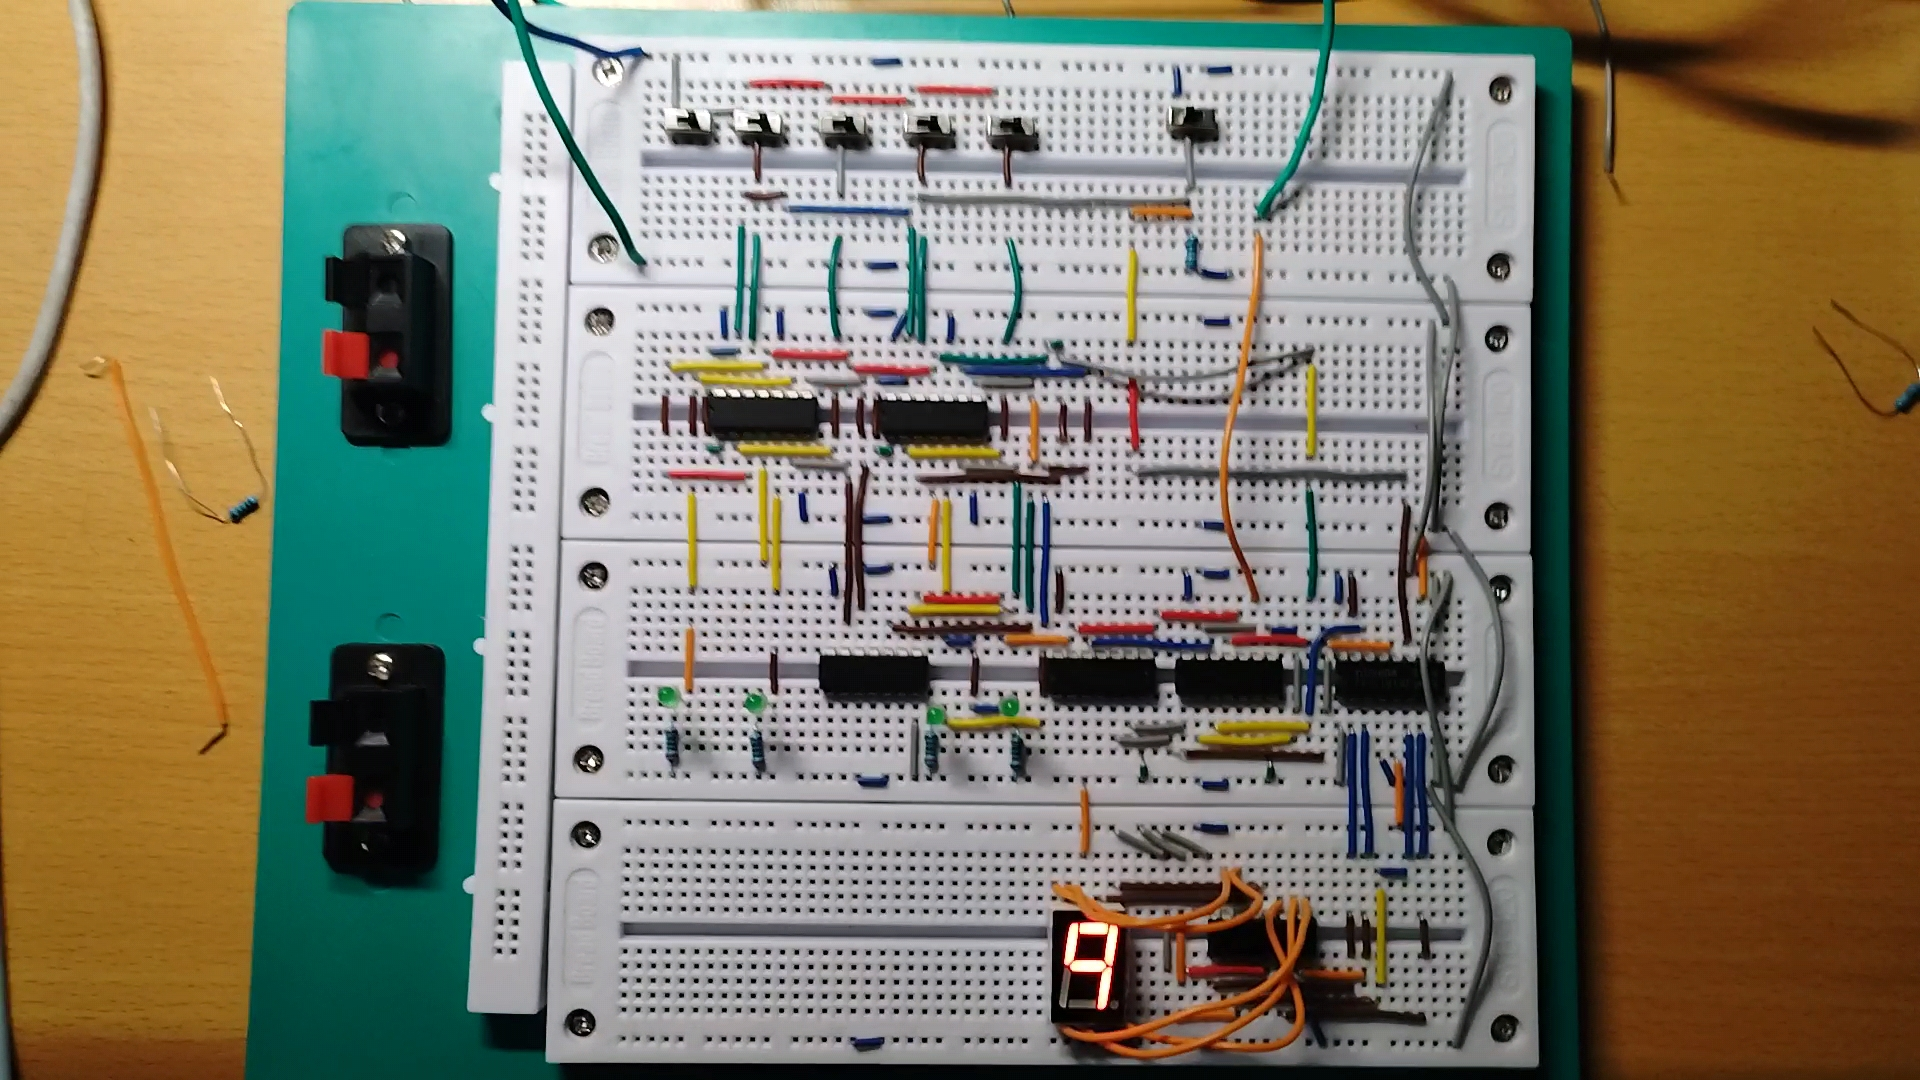
\includegraphics[width=0.8\textwidth]{复位状态.jpg}
           \caption{复位状态}
    \label{7474}
    \end{minipage}
\end{figure}
\begin{figure}[H]
    \centering
    \begin{minipage}{0.45\textwidth}
        \centering
               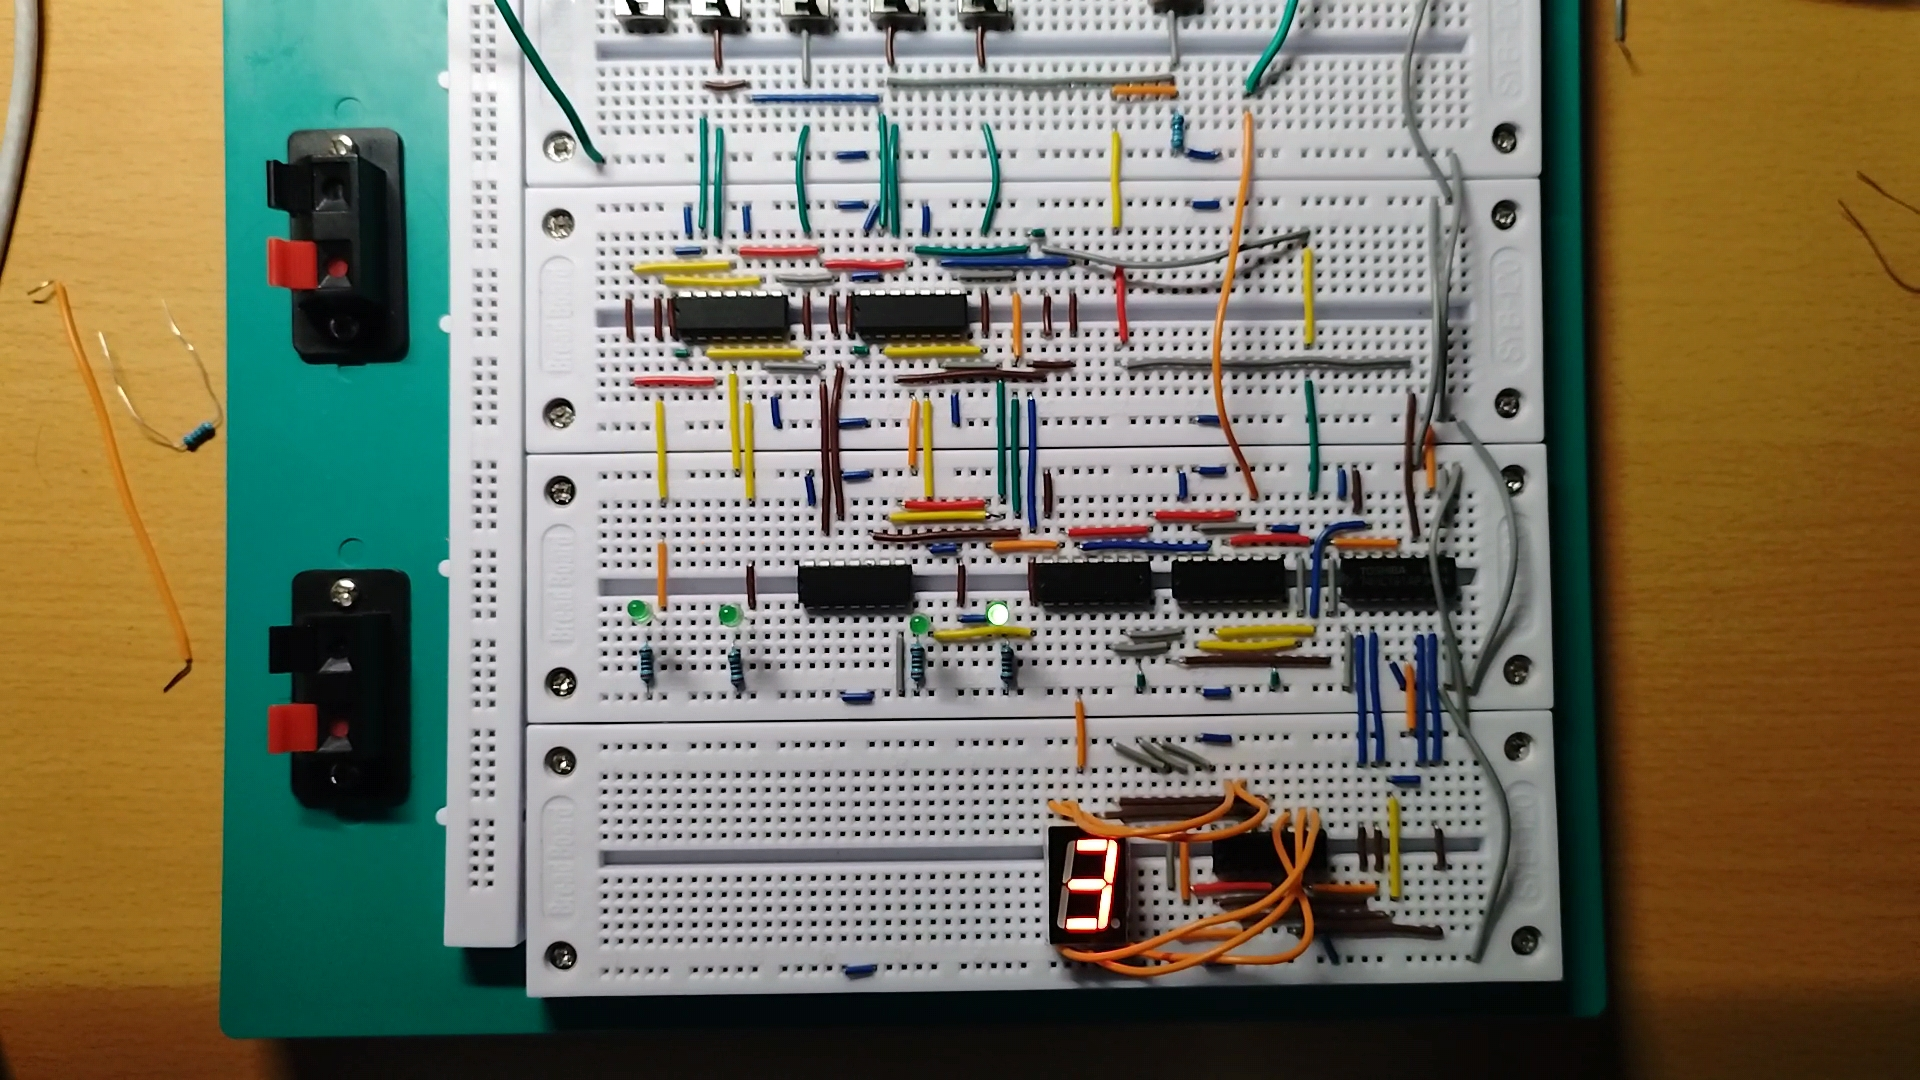
\includegraphics[width=0.8\textwidth]{计时中.jpg}
               \caption{抢答成功并计时}
        \label{7474}
        \end{minipage}
        \hspace{0.05\textwidth}
    \begin{minipage}{0.45\textwidth}
    \centering
           \includegraphics[width=0.8\textwidth]{计时结束.jpg}
           \caption{计时结束}
    \label{计时结束}
    \end{minipage}    
\end{figure}
在最开始的设计中,没有考虑计时结束之后的问题,计时器会从最高位重新开始计数,会出现伪码显示错误的数字。为了消除这一错误,利用计数器的$MIN$输出端,当计时到0后$MIN$端出1,用这个信号取非后再与原来的时钟信号相与非,可以屏蔽计数结束之后的时钟信号,进而让显示器保持在0位置。图\ref{计时结束}是修改后的电路,当计时结束后显示器始终保持在0,且不影响其他功能,说明修改有效。
\section{反思与总结}
在设计消抖电路时最开始遇到两个问题。一是没有意识到电阻的重要性,而且两个与非门要单独接电阻而不能共用一个电阻。电源直接短路到地导致造成仿真出错;二是对功能的理解出现偏差。要屏蔽其他输入,首先想到的是利用优先编码器,但是这种屏蔽是“不对称”的,即若A的优先级比B高,那么即使B先于A按下抢答按钮,最终也会显示A灯亮而B灯不亮,这显然与实际抢答过程不符,因此不能使用优先编码器。

七段数码管的高电平不能接5V,会超出正常工作电压范围。仿真时一直无法正确显示数码,通过上网查阅数码管手册才得以解决。
\end{document}